%%%%%%%%%%%%%%%%%%%%%%%%%%%%%%%%%%%%%%%%%%%%%%%%%%%%%%%%%%%%%%%%%%%%%%%%%
%
%      VTU Project-report Template using LaTeX  
%      Copyright 2011 shashi <shashi859@gmail.com>,
%	ashish <ashishsram@gmail.com>
%      
%      This program is FREE SOFTWARE; you can redistribute it and/or modify
%      it under the terms of the GNU General Public License as published by
%      the Free Software Foundation; either version 2 of the License, or
%      (at your option) any later version.
%      
%      This program is distributed in the hope that it will be useful,
%      but WITHOUT ANY WARRANTY; without even the implied warranty of
%      MERCHANTABILITY or FITNESS FOR A PARTICULAR PURPOSE.  See the\abstractintoc
\thispagestyle{plain}
\renewcommand{\abstractname}{Abstract}
\renewcommand{\abstractnamefont}{\Large\textbf}
\renewcommand{\abstracttextfont}{\normalsize}
\begin{abstract}
\OnehalfSpacing

{\LaTeX} eases our pressure in writing thesis \& reports because of its powerful features such as automatic hyphenation, table of contents, figures & tables,  powerful bibliography tool, citations,Automatic Numbering of Chapter, sections, figures & tables, its beautiful fonts, professional output...

Writing too much of code for gives bad impression on {\LaTeX}. But now we have numerous gui tools like gedit-latex-plugin, {\TeX}maker, Lyx & emacs, which are very much user friendly. 

This VTU-project-report-template is written using popular document class, ``Memoir". In the coming chapters, we hav given small help manual required for writing report & at the end about template

\end{abstract}

%      GNU General Public License for more details.
%      
%      You should have received a copy of the GNU General Public License
%      along with this program; if not, write to the Free Software
%      Foundation, Inc., 51 Franklin Street, Fifth Floor, Boston,
%      MA 02110-1301, USA.

\documentclass[12pt,a4paper,oneside]{memoir}%Memoir is more versatile than other document classes like article, report, book etc,
\usepackage{graphicx}%to handle image, like scaling
\usepackage[english]{babel}
\usepackage[a4paper,right=1in]{geometry}%used for modifying page layout
\usepackage[hidelinks]{hyperref}%for referencing contents,figure,table...
\usepackage{listings}%for including source code
\usepackage{pdfpages}%to attach pdf files
\usepackage{fancyvrb} % Verbatim
\usepackage[section,subsection,subsubsection]{extraplaceins} % Required to force a figure to be within sections, subsectons, subsubsections
%document starts here
\begin{document}

\begin{titlepage}
%\clearpage
\thispagestyle{empty}\centering
\newlength{\toptafiddle} 
\newlength{\bottafiddle}

\setlength{\toptafiddle}{1in}
\setlength{\bottafiddle}{1in}
\vspace*{-0.75in}
\enlargethispage{\toptafiddle}
\textbf{\HUGE LAB REPORT}\vfill % \textbf{\Huge of} \\

%Affiliated to\\
%\textbf{Kerala Technical University  (KTU), Trivandrum}\\

\vspace{0.2cm}
\begin{figure}[h]
\centering
%
\includegraphics[height=4cm]{images/ktu.jpg}
%\hspace{0.1\textwidth}

\includegraphics[height=3.7cm]{images/cem1.png}
\end{figure}

\vfill

\Huge{\textbf{04 EC 6593 DESIGN LAB - I}}
\vfill

\large Lab Report  submitted in partial fulfillment of the curriculum
prescribed for the award  of Master of Technology degree
in \vfill \textbf{\Large Electronics \& Communication Engineering}  \vfill with specialization in \vfill
\textbf{\Large VLSI and Embedded Systems} \vfill by\vfill


\begin{tabular}{ccc}
4JC11EC0 &  & Student-1\\
4JC11EC0 &  & Student-2\\
4JC11EC0 &  & Student-3\\
4JC11EC0 &  & Student-4\\
\end{tabular}
\vfill
%Under the Guidance of\vfill
%
%
%\textbf{Jayakrishnan K. R.}\\
%\textbf{Asst. Professor}\\
%\textbf{Department of ECE, CoE, Munnar}
%\vfill


%\vfill
%\textbf{\small DEPARTMENT OF ELECTRONICS \& COMMUNICATION ENGINEERING}
\vfill
%Affiliated to \vfill

\textbf{\large NOVEMBER 2015}\vfill
 \textbf{\Large COLLEGE OF ENGINEERING MUNNAR} \vfill
 \textbf{\Large (APJ Abdul Kalam Technological University)} \vfill
 \textbf{\large P.B. No. 45, County Hills, %} \vfill \textbf{\Large 
 Munnar, Kerala - 685612} \vfill
\end{titlepage}
%include titlepage,i.e, title.tex file

%Page layout according to VTU specification
%Right=1.25in,left=1in, Top & Bottom 0.75in in each

\setlength{\oddsidemargin}{0.25in}%left side margin{1in by default+0.25in}

%header specification
\setlength{\headheight}{\onelineskip}
\setlength{\headsep}{6pt}
\setlength{\topmargin}{-0.25in}

%footer specification
\setlength{\footskip}{\onelineskip}
\setlength{\footnotesep}{\onelineskip}

%A4 paper height = 11.69in
%thus 11.69in-9.67in-1in(top+header) is approx 0.75in left for bottom
\setlength{\textheight}{9.67in}

\brokenpenalty=10000% Disallow page breaks at hyphens

\OnehalfSpacing

\newlength{\toptafiddle} 
\newlength{\bottafiddle}
%
\setlength{\toptafiddle}{1in}
\setlength{\bottafiddle}{1in}
\vspace*{-0.5in}
\enlargethispage{\bottafiddle}
\thispagestyle{empty}

\begin{center}\large \\\textbf{\Large COLLEGE OF ENGINEERING MUNNAR}\\ \textbf{\Large P.B. No. 45, County Hills, Munnar - 685612} \vfill
 Affiliated to\\
\textbf{APJ Abdul Kalam  Technological University}\\
\vspace{0.2cm}
\begin{figure}[h]
\centering
%
\includegraphics[height=4cm]{images/ktu.jpg}
%\hspace{0.1\textwidth}

\includegraphics[height=3.7cm]{images/cem1.png}
\end{figure}\\
\Huge{Certificate}\end{center}

This is to certify that the work entitled ``04 EC 6593 DESIGN LAB -I'' is a bonafide record of work carried out by Student-1 in partial fulfillment of the requirements for the  award of the degree of Master of Technology in Electronics \& Communication Engineering with specialization in VLSI and Embedded Systems of APJ Abdul Kalam Technological University, during the year 2015-2017. 

\vfill
\begin{minipage}[t]{0.5\textwidth}%
\emph{Staff in Charge}\\
Jayakrishnan K. R. \\
Asst. Professor\\
Department of ECE\\
CoE, Munnar 685612
\end{minipage}\hspace{2cm}
\begin{minipage}[t]{0.4\textwidth}%
{\emph{Head of the Department}}\\
Ramesh P. \\
Associate Professor and Head\\
Department of ECE\\
CoE, Munnar 685612
\end{minipage}

\vfill
\begin{minipage}[t]{0.3\textwidth}%
\begin{tabular}{lcc}
 &  & \tabularnewline
 &  & \tabularnewline
 &  & \tabularnewline
Date & : & \tabularnewline
Place &: & Munnar\tabularnewline
\end{tabular}%
\end{minipage}\hspace{2cm}
\begin{minipage}[t]{0.4\textwidth}%
\noindent %
\begin{tabular}{ccr}
Examiners & :& 1.\_\_\_\_\_\_\_\_\_\_\_\_\_\_\_\_\_\_\_\_\_\_\_\_\_\\
&  & \\
&  & 2.\_\_\_\_\_\_\_\_\_\_\_\_\_\_\_\_\_\_\_\_\_\_\_\_\_\\
 &  & \\
&  & 3.\_\_\_\_\_\_\_\_\_\_\_\_\_\_\_\_\_\_\_\_\_\_\_\_\_\\
\end{tabular}%
\end{minipage}

\pagenumbering{roman}
\pagestyle{plain}
\renewcommand{\abstractname}{Acknowledgement}
\renewcommand{\abstractnamefont}{\Large\textbf}
\renewcommand{\abstracttextfont}{\normalsize}
\begin{abstract}
\OnehalfSpacing
%An endeavour is successful only when it is carried out under proper guidance \& blessings. We would like to thank few people who helped us in carrying out this work by lendind invaluable assistance to us in carrying out this work by lending invaluable assiatance to us.\\
%
%We are hereby thankful to Dr B.G.Sangameshwara, Principal SJCE, Mysore \& Dr C.R Venugopal, HOD of E\&C, SJCE, Mysore who encouraged at this venture
%
%We sincerely thank Dr Sudarshan Patilkulkarni, Assistant Professor Dept Of E\&C, SJCE, Mysore for constructive \& encouraging suggestions.
%
%We also thank all Teaching & Non-teaching staff of E\&C Dept SJCE, Mysore for their kind of co-operation during our course
%
%Finally we are extremely thankful to our Family \& Friends who helped us in our work \& made the project a successful one.

``\textbf{Acknowledgement} - This is where you thank all those people whom you've rarely (or never) met but whose inspiration, motivation, encouragement, blessings etc. etc. have helped u to write this immensely knowledgeable report and NOT thank your friend who did most of your coding. There is some debate as to whether Abstract should come first or Acknowledgement. I don't care bcz VTU doesnt seem to care. I wrote it this way and it was accepted ... that's all that matters."
--\textbf{writes Basavraj Talwar} in his website, a jce alumni & currently in IISc, who has also written \LaTeX-vtu-template

But for preparing this template Anandmurthy Sir of EEE motivated us \& gave guidance & some suggestions from CRN

And great thanks for Memoir-Document class manual which tells almost all things, which u want while writing a report.

\vspace{3cm}
\begin{flushleft}Ashish\\Shashi\end{flushleft}
\vfill
\end{abstract}


\setcounter{secnumdepth}{2}%sections numbering upto 2 level.i.e,chapter,section,subsection & any later sections will not be numbered
\renewcommand{\contentsname}{Table of Contents}
\hypersetup{%
    pdfborder = {0 0 0}
}

\tableofcontents
\pagebreak

\listoffigures
\pagebreak
\listoftables 
\pagebreak

\abstractintoc
\thispagestyle{plain}
\renewcommand{\abstractname}{Abstract}
\renewcommand{\abstractnamefont}{\Large\textbf}
\renewcommand{\abstracttextfont}{\normalsize}
\begin{abstract}
\OnehalfSpacing

{\LaTeX} eases our pressure in writing thesis \& reports because of its powerful features such as automatic hyphenation, table of contents, figures & tables,  powerful bibliography tool, citations,Automatic Numbering of Chapter, sections, figures & tables, its beautiful fonts, professional output...

Writing too much of code for gives bad impression on {\LaTeX}. But now we have numerous gui tools like gedit-latex-plugin, {\TeX}maker, Lyx & emacs, which are very much user friendly. 

This VTU-project-report-template is written using popular document class, ``Memoir". In the coming chapters, we hav given small help manual required for writing report & at the end about template

\end{abstract}

%creating custom header & footer. Look into memoir manual for details
\pagestyle{myheadings}
\makeheadrule{myheadings}{\textwidth}{0.4pt}
\makefootrule{myheadings}{\textwidth}{0.4pt}{}
\makeoddhead{myheadings}{\small{Lab Report of  04 EC 6593 Design Lab - I }}{}{\small{Chapter \thechapter}}
\makeoddfoot{myheadings}{\small{Dept of ECE, CoE, Munnar}}{}{\small{\thepage}}

\pagenumbering{arabic}

\part{VLSI Experiments}
\chapter{Digital Experiments}
\section{Combinational Circuits}

\subsection{Full Adder}

\subsection*{Aim}

To design and synthesize  a full adder using  verilog and verify its functionality using RTL and Gate Level Simulation and to draw its layout.  Also find the area consumed, power and delay of the full adder.

\subsection*{Program}
\subsubsection*{Full Adder Source}
\begin{Verbatim}

/***************************************************************************
				FULL ADDER	
***************************************************************************/
`timescale 1ns / 1ps
module full_adder(x,y,cin,sum,cout);

	input x,y,cin;
	output sum,cout;
	
	assign sum=(x^y)^cin;
	assign cout=(x&y)|(x&cin)|(y&cin);
	
endmodule

\end{Verbatim}
\pagebreak


\paragraph{Full Adder Testbench}

\begin{Verbatim}
/***************************************************************************
				FULL ADDER - TESTBENCH
***************************************************************************/
`timescale 1ns / 1ps
module full_adder_tb;

	// Inputs
	reg x;
	reg y;
	reg cin;

	// Outputs
	wire sum;
	wire cout;

	// Instantiate the Unit Under Test (UUT)
	full_adder uut (
		.x(x), 
		.y(y), 
		.cin(cin), 
		.sum(sum), 
		.cout(cout)
	);

	initial begin
		// Initialize Inputs
		
		//Case 0 : 0+0 with carry in of 0
		x = 0;
		y = 0;
		cin = 0;

		// Wait 100 ns for global reset to finish
		#100;
        
		// Add stimulus here
		
		//Case 0 : 0+0 with carry in of 1
		x = 0;
		y = 0;
		cin = 1;
		#20; 
		
		//Case 0 : 0+1 with carry in of 0
		x = 0;
		y = 1;
		cin = 0;
		#20;
		
		//Case 0 : 0+1 with carry in of 1
		x = 0;
		y = 1;
		cin = 1;
		#20;
		
		//Case 0 : 1+0 with carry in of 0
		x = 1;
		y = 0;
		cin = 0;
		#20;
		
		//Case 0 : 1+0 with carry in of 1
		x = 1;
		y = 0;
		cin = 1;
		#20;
		
		//Case 0 : 1+1 with carry in of 0
		x = 1;
		y = 1;
		cin = 0;
		#20;
		
		//Case 0 : 1+1 with carry in of 1
		x = 1;
		y = 1;
		cin = 1;
		#20;
	
	end
      
endmodule
\end{Verbatim}


\subsection*{Outputs}

\subsubsection*{RTL Simulation}
\FloatBarrier
\begin{figure}[!hp]
\centering
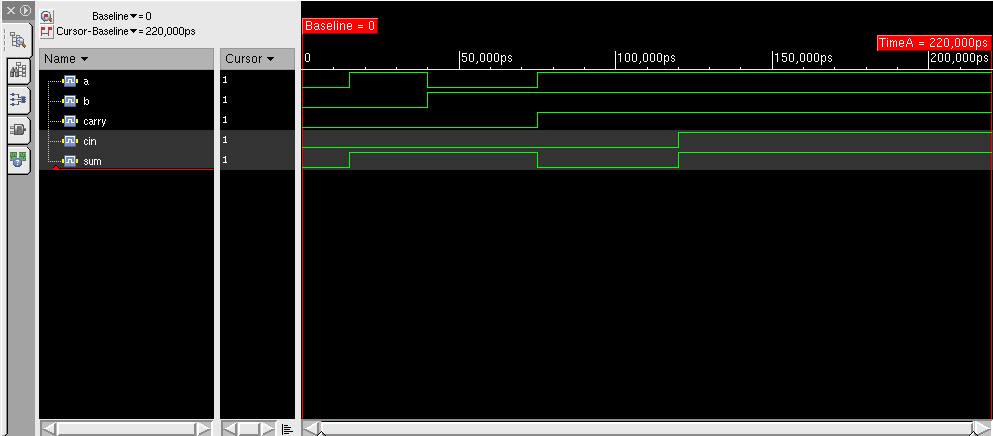
\includegraphics[width=0.9\textwidth]{images/rtl.png}
\caption{RTL Simulation of Full Adder}
\end{figure}

\pagebreak

\subsubsection*{Synthesized Top Level Schematic}
\FloatBarrier
\begin{figure}[!hp]
\centering
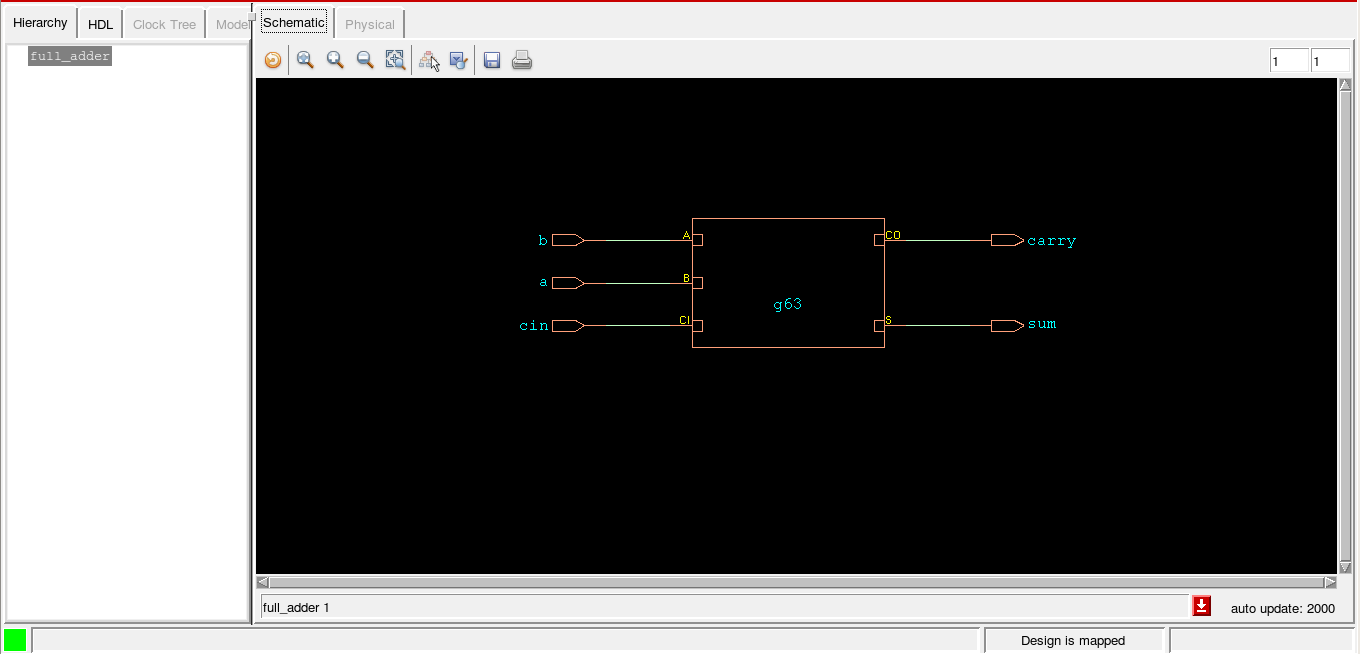
\includegraphics[width=0.9\textwidth]{images/toplevel.png}
\caption{Synthesized Top Level Schematic of Full Adder}
\end{figure}

\subsubsection*{Total Area consumed}
\FloatBarrier
\begin{figure}[!hp]
\centering
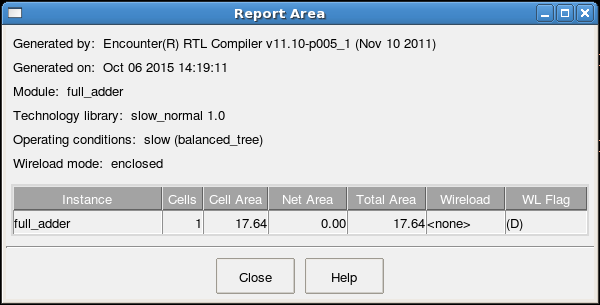
\includegraphics[width=0.9\textwidth]{images/area.png}
\caption{Total Area consumed by Full Adder}
\end{figure}
\pagebreak

\subsubsection*{Total Area consumed}
\FloatBarrier
\begin{figure}[!htpb]
\centering
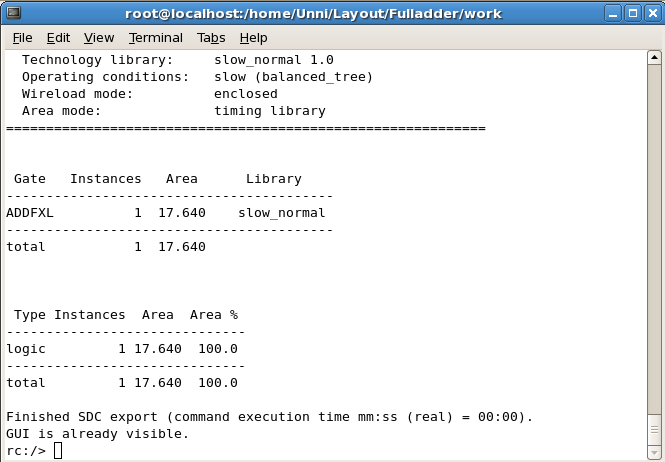
\includegraphics[width=0.8\textwidth]{images/areartl.png}
\caption{Total Area consumed by Full Adder shown in Terminal}
\end{figure}

\subsubsection*{Worst Path Delay}
\FloatBarrier
\begin{figure}[!htpb]
\centering
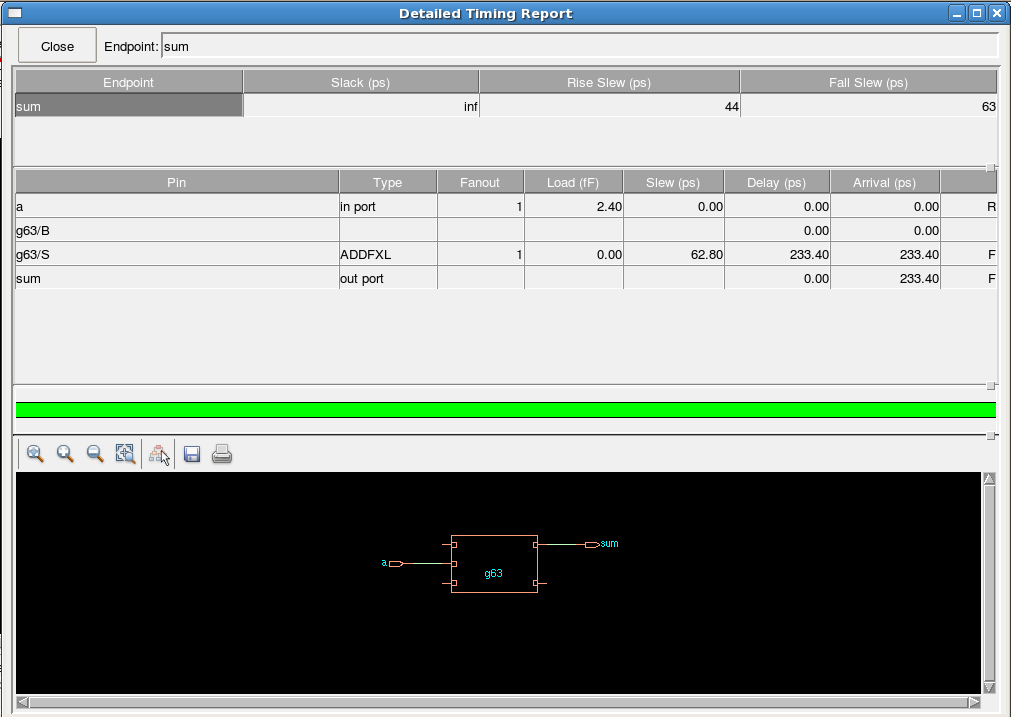
\includegraphics[width=0.9\textwidth]{images/worstpath.png}
\caption{Worst Path Delay of Full Adder}
\end{figure}

\subsubsection*{Power Consumed}
\FloatBarrier
\begin{figure}[!htpb]
\centering
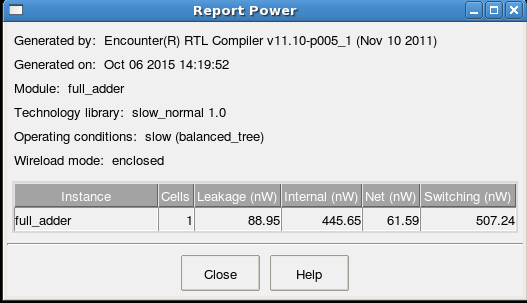
\includegraphics[width=0.7\textwidth]{images/power.png}
\caption{Power Consumed by Full Adder}
\end{figure}

\subsubsection*{Layout}
\FloatBarrier
\begin{figure}[!htpb]
\centering
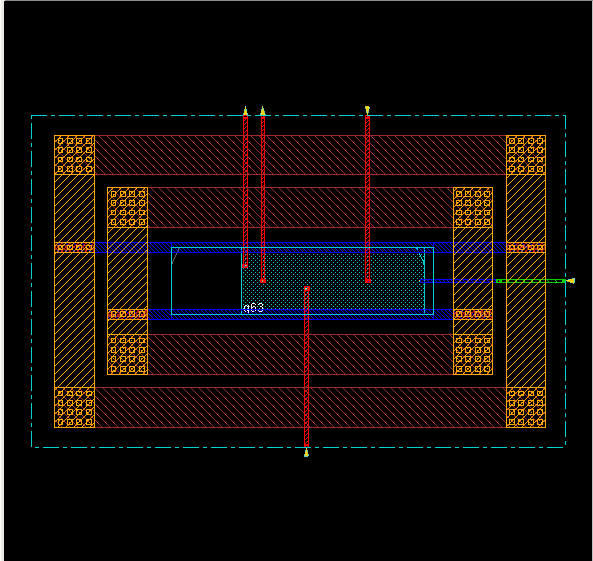
\includegraphics[width=0.8\textwidth]{images/layout.png}
\caption{Layout of Full Adder}
\end{figure}

\subsubsection*{Area Consumed in Layout}
\FloatBarrier
\begin{figure}[!htpb]
\centering
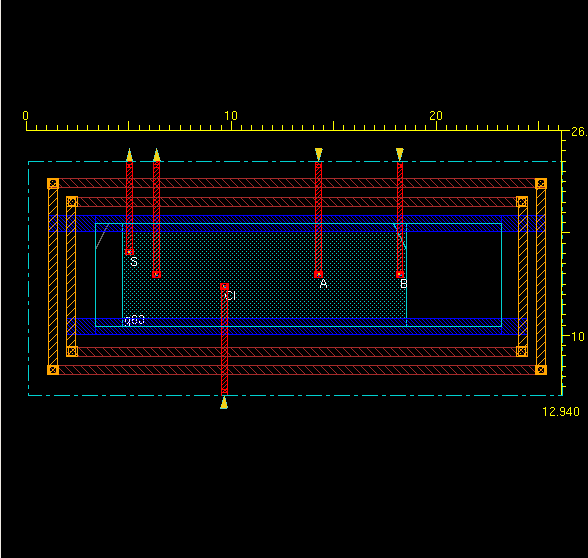
\includegraphics[width=0.8\textwidth]{images/layoutarea.png}
\caption{Area Consumed by Full Adder in Layout}
\end{figure}

\subsubsection*{Gate Level Simulation}
\FloatBarrier
\begin{figure}[!htpb]
\centering
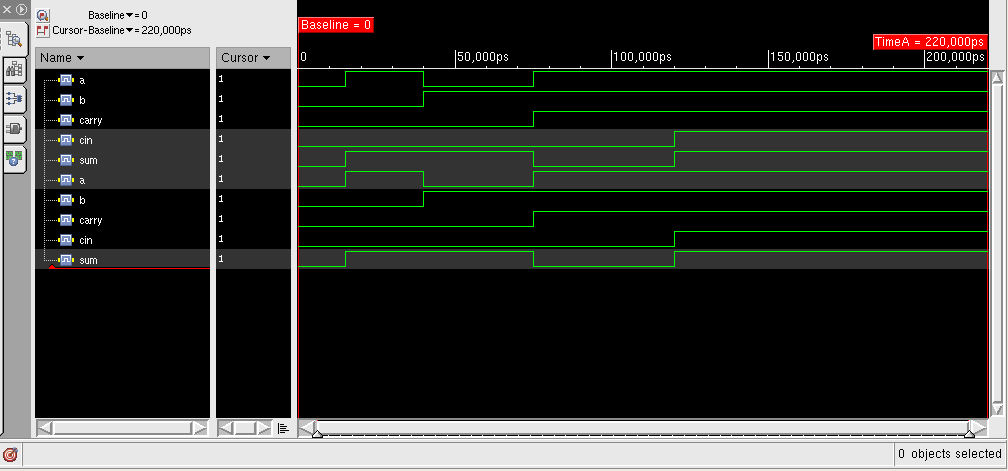
\includegraphics[width=0.9\textwidth]{images/gatelevel1.png}
\caption{Gate Level Simulation of Full Adder}
\end{figure}



\subsection*{Result}

Designed and synthesized  a full adder using  verilog and verified its functionality using RTL and Gate Level Simulation and also drawn its layout.  The area, power and delay of full adder is found out.



\subsection{Project Organization}
	The project is split-up into 6 stages as shown in table :\\
	
\begin{tabular}{|c|c|c|}\hline
Sl No&Work& Duration(in Weeks)\\ \hline \normalsize
1&Information Collection on DFB \& VNC&1 \\ \hline
2&Information collection on development tools&2\\ \hline
3&Integrating DirectFB \& VNC&8\\ \hline
4&Cross Compiling \& Porting&2\\ \hline
5&Building JPEG libraries&2\\ \hline
6&Testing&2\\ \hline
\end{tabular}



%\include{chapter2}
%\include{chapter3}
%\include{chapter4}
\include{reference}
%%\addappheadtotoc
%\begin{appendices}
%\chapter{ATMega 8}%this wil by default adds Appendix A,B,C...you can specify ur own name like \chapter{Datasheets}
%Here is the datasheets of various ATmega8
%\includepdf[pages=1-10]{pdf/atmega8.pdf}%here it appends only 3 pages
%
%\end{appendices}

\end{document}
